\section{Comparision between LNLT\_shell and NuShellX}
% Displaying the eigne values of each program side by side.
% comment on that we compute more states than nushellx computes.
% display the occupation numbers

To verify that the code described in the previous section works, several isotopes of oxygen were computed with LNLT\_shell and compared to the result from NuShellX with the USDB interaction. In table \ref{tab:ox18},\ref{tab:ox19} and \ref{tab:ox20} the eigenenergies of \(^{18,19,20}\rm{O}\) are compared to the values computed with NuShellX. The energies are relative the ground energy of \(^{16}\rm{O}\). There are almost no difference to the given numerical precission, only a few of the higher eigen-values differ slightly. In addition the code seems to correctly assign total angular momentum; the \(J_L\) columns are identical with the \(J_N\) columns. To illustrate the similarity further, the lowest energies are plotted in figure \ref{fig:ox18eig},\ref{fig:ox19eig} and \ref{fig:ox20eig}, where also a comparision to experiment is made.

\onecolumngrid

\begin{figure}[h!]
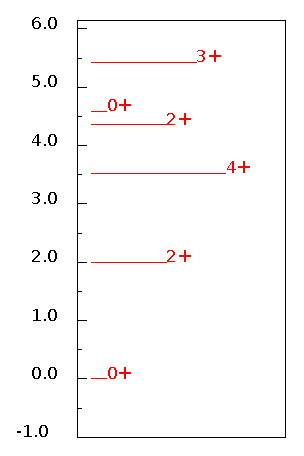
\includegraphics{ox18.eps}
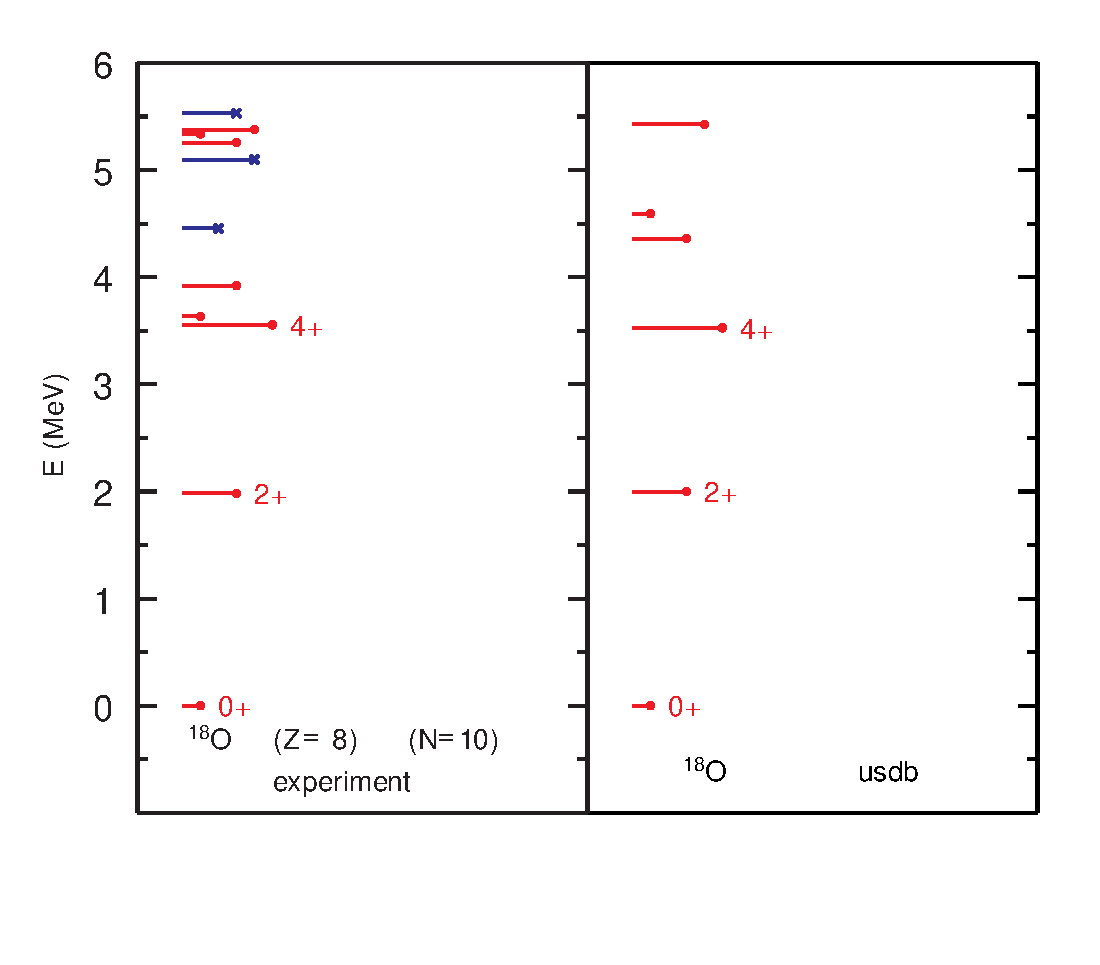
\includegraphics[scale=0.56,trim=0cm 2.3cm 0cm 0cm]{o_18b.eps}
\caption{The lowest energy states of $^{18}\rm{O}$, computed by LNLT\_shell to the left compared to the eigenspectrum from experiment and NuShellX to the right}
\label{fig:ox18eig}
\end{figure}

\begin{figure}[h!]
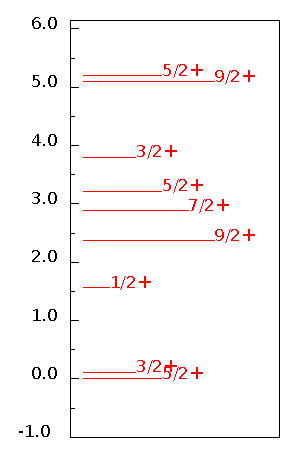
\includegraphics{ox19.eps}
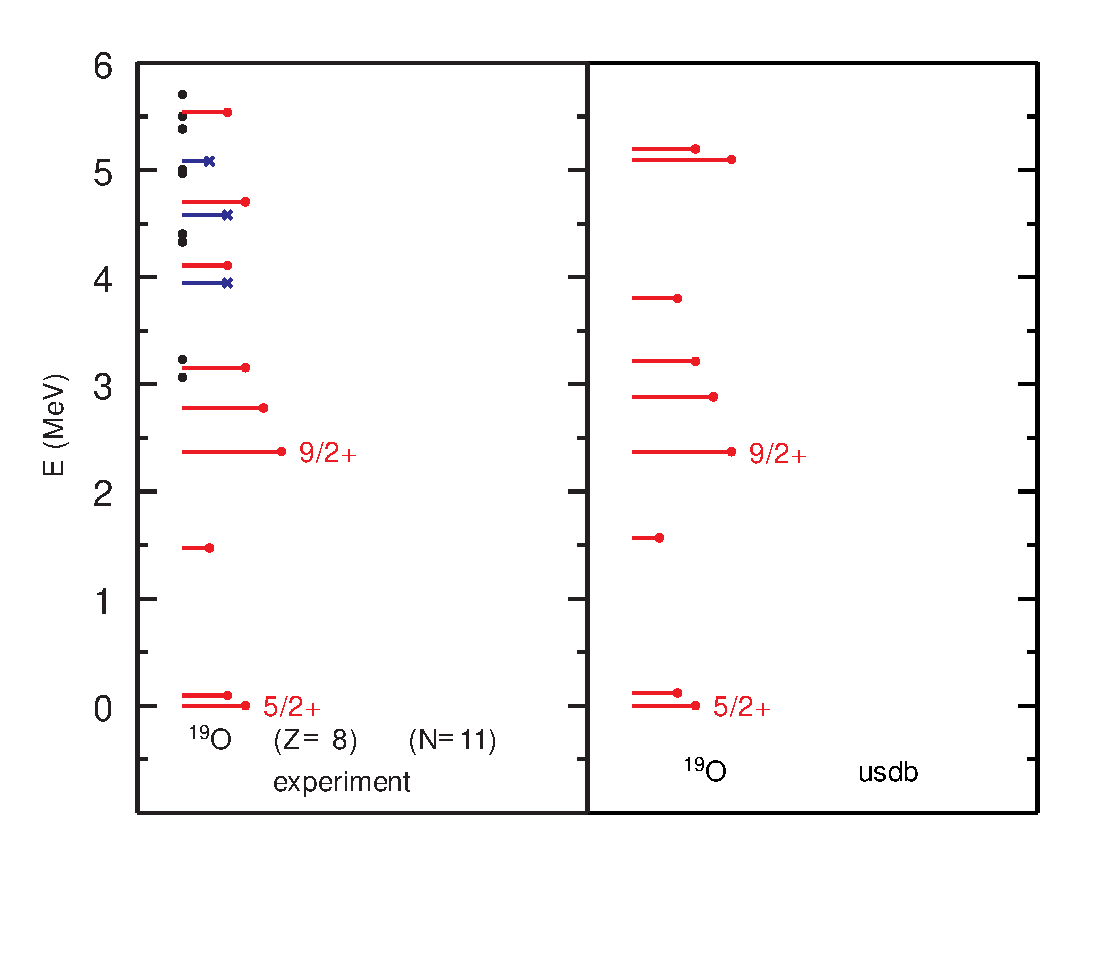
\includegraphics[scale=0.56,trim=0cm 2.3cm 0cm 0cm]{o_19b.eps}
\caption{The lowest energy states of $^{19}\rm{O}$, computed by LNLT\_shell to the left compared to the eigenspectrum from experiment and NuShellX to the right}
\label{fig:ox19eig}
\end{figure}

\begin{figure}[H]
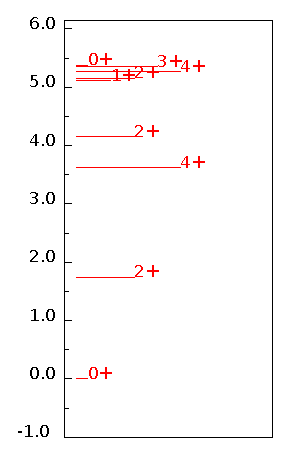
\includegraphics{ox20.eps}
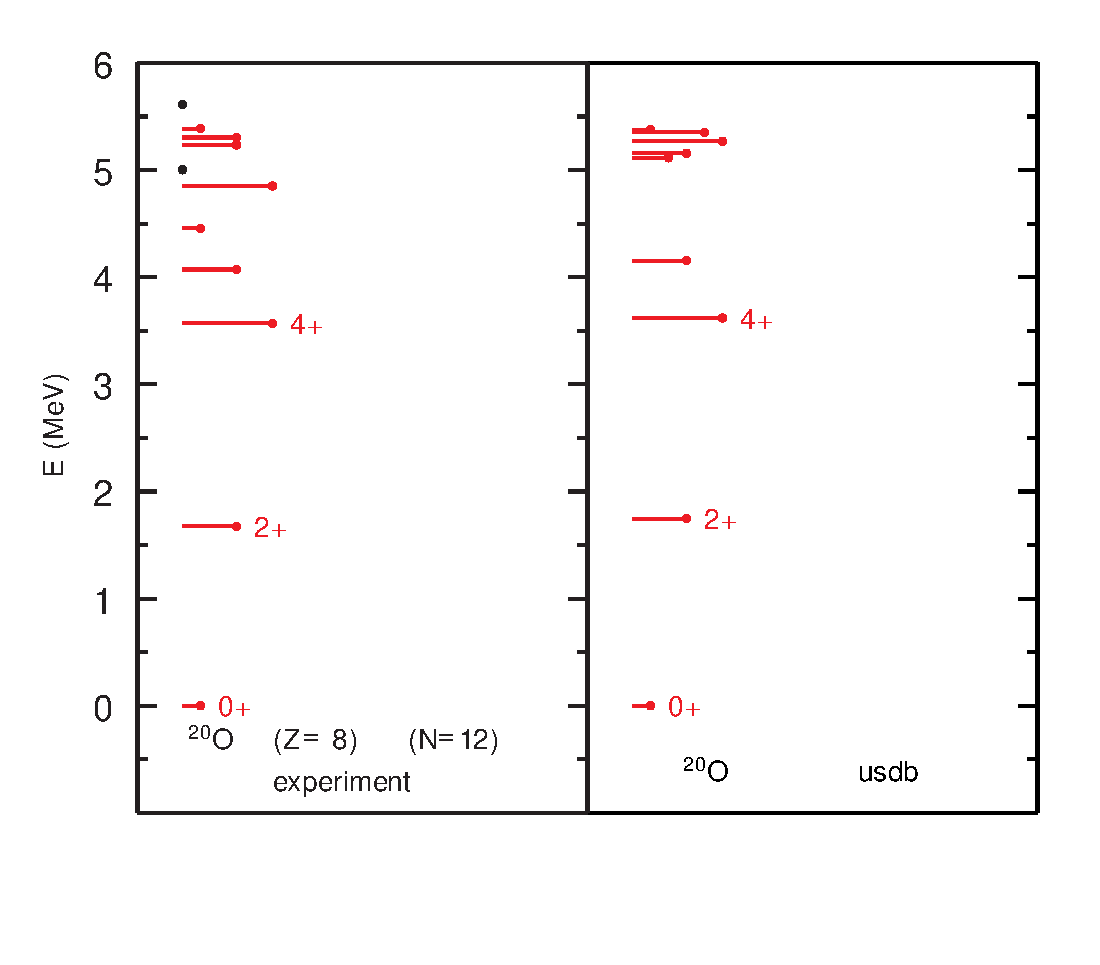
\includegraphics[scale=0.56,trim=0cm 2.3cm 0cm 0cm]{o_20b.eps}
\caption{The lowest energy states of $^{20}\rm{O}$, computed by LNLT\_shell to the left compared to the eigenspectrum from experiment and NuShellX to the right}
\label{fig:ox20eig}
\end{figure}

\twocolumngrid

In addition to the eigen-spectrum for each isotope shell-occupation numbers were also computed. In Table \ref{tab:ox18occ} all the shell-occupation numbers for all \(14\) states can be viewed, computed both with LNLT\_shell and with NuShellX. There are some slight difference, however this can be easily explained with that LNLT\_shell outputs higher precision than NuShellX does and thus the difference is most likely due to rounding errors. In Figs. \ref{fig:occnum_lnlt} and \ref{fig:occnum_nushellx} the shell occupation for the ground state and the first excited states are visualized, computed by LNLT\_shell and NuShellX respectively. Also here there are a slight differences, which still can be explained with rounding errors. \\

\onecolumngrid

\begin{figure}[H]
  \begin{center}
  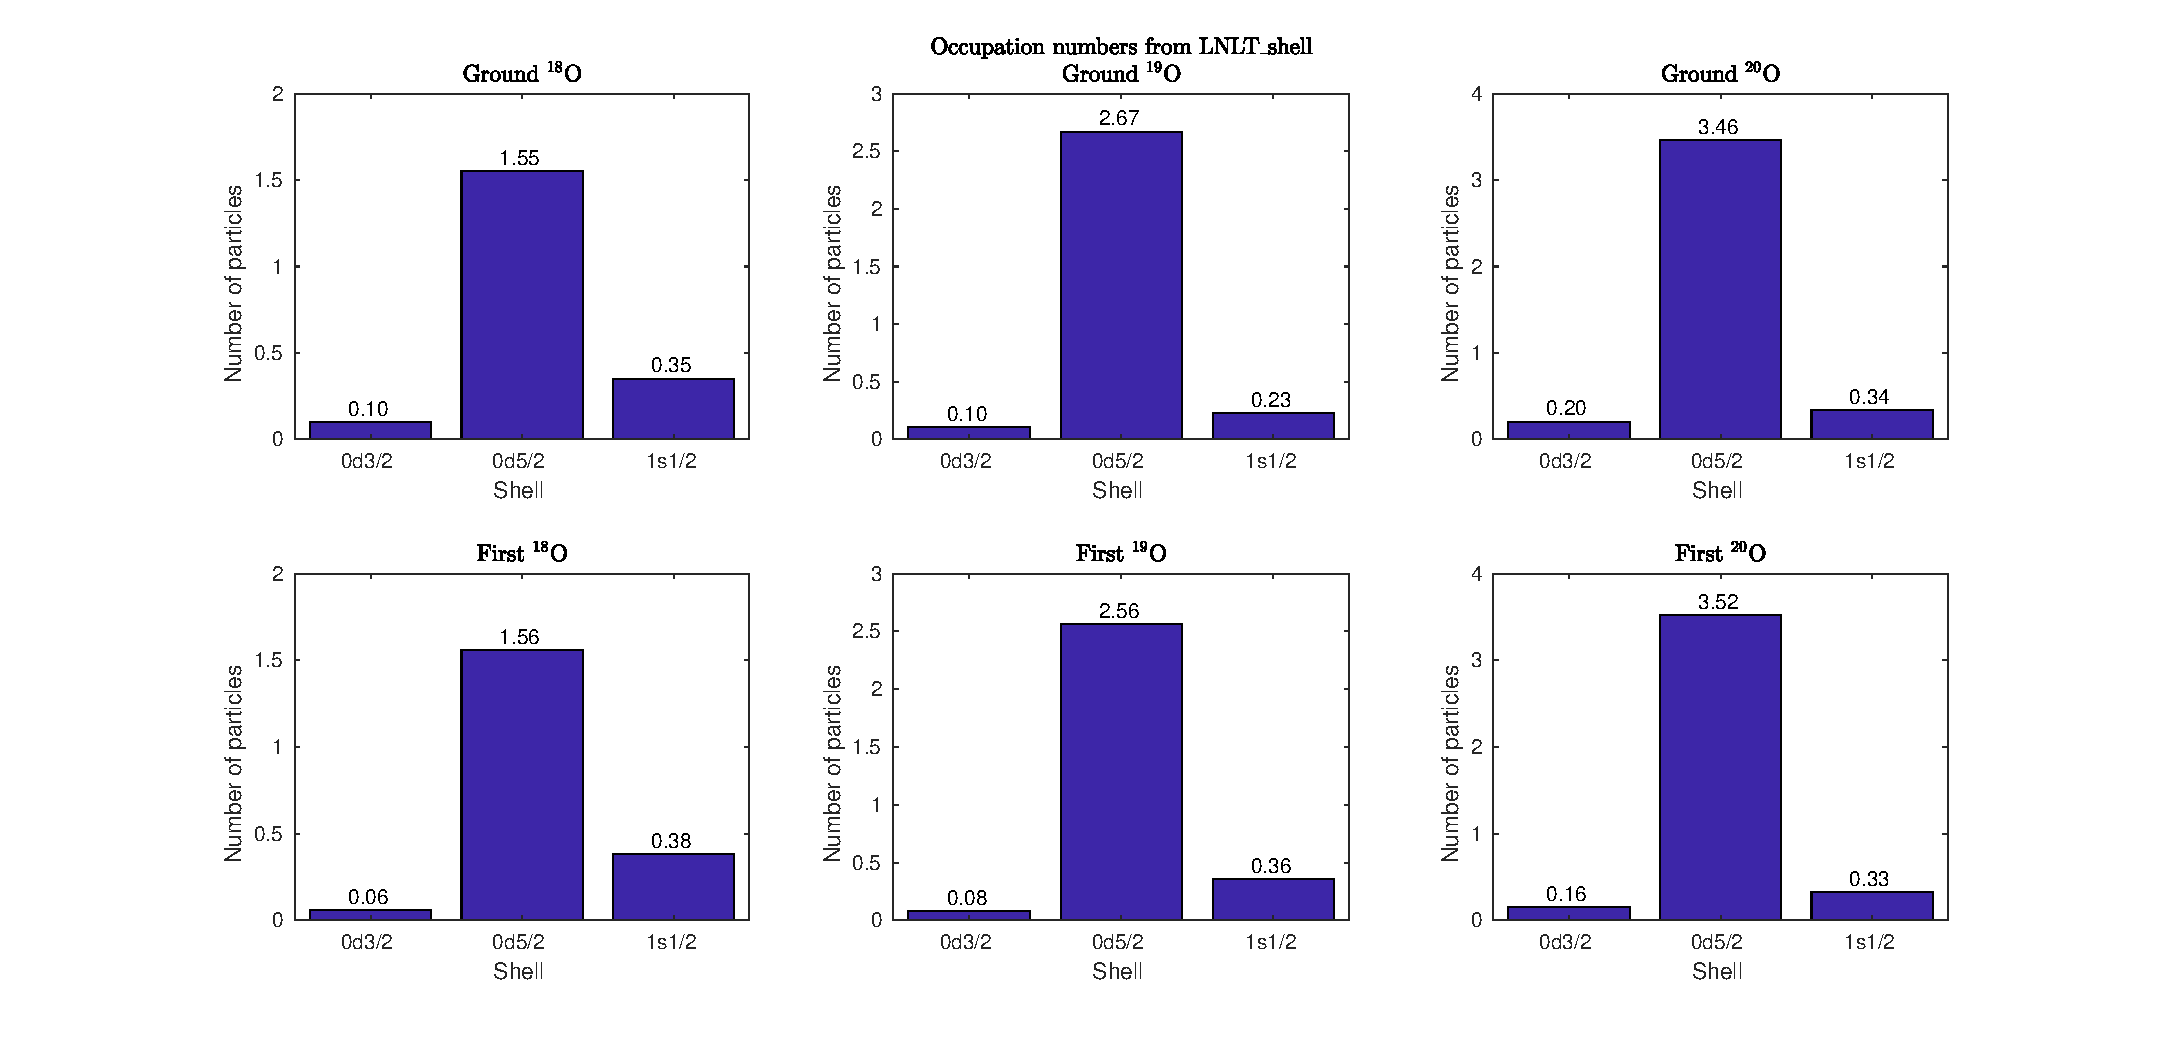
\includegraphics[scale=0.5]{occupation_numbers_lnlt.eps}
  \caption{The occupation numbers of the ground state and first excited state of \(^{18,19,20}\rm{O}\) as computed by LNLT\_shell.}
  \label{fig:occnum_lnlt}
  \end{center}
\end{figure}

\begin{figure}[H]
  \begin{center}
  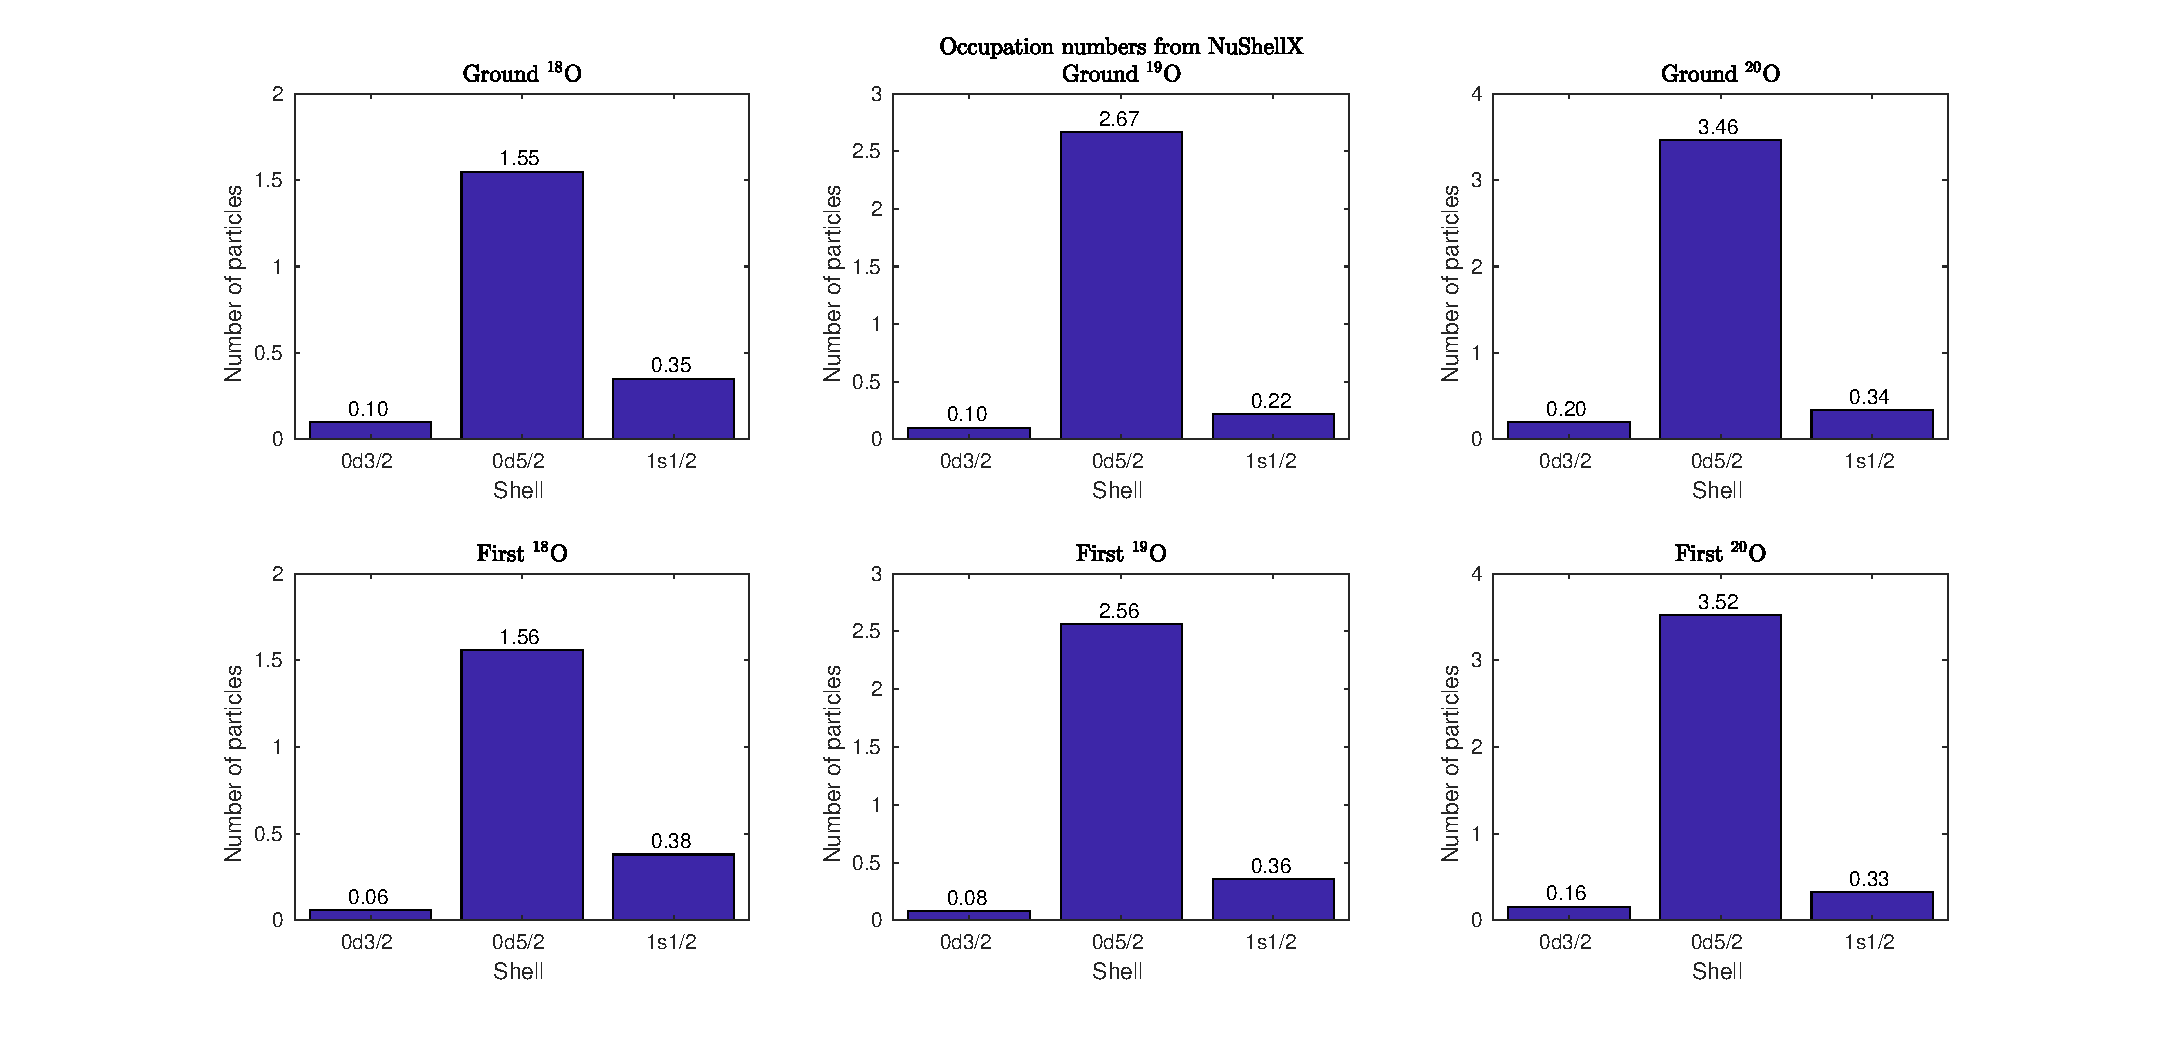
\includegraphics[scale=0.5]{occupation_numbers_nushellx.eps}
  \caption{The occupation numbers of the ground state and first excited state of \(^{18,19,20}\rm{O}\) as computed by NuShellX.}
  \label{fig:occnum_nushellx}
  \end{center}
\end{figure}

\twocolumngrid
